\documentclass[12pt,a4paper]{article}

% Packages
\usepackage[utf8]{inputenc}
\usepackage[margin=1in]{geometry}
\usepackage{amsmath,amssymb,amsthm}
\usepackage{graphicx}
\usepackage{booktabs}
\usepackage{algorithm}
\usepackage{algpseudocode}
\usepackage{hyperref}
\usepackage{cite}
\usepackage{float}
\usepackage{subcaption}
\usepackage{multirow}
\usepackage{tabularx}

% Hyperref setup
\hypersetup{
    colorlinks=true,
    linkcolor=blue,
    filecolor=magenta,      
    urlcolor=cyan,
    citecolor=blue
}

% Title information
\title{\textbf{Comparative Analysis of Heuristic Algorithms for the Multidimensional Knapsack Problem}}
\author{
    \textbf{Omega Group 9} \\[0.5em]
    Shovon Roy (2005010), Tusher Bhomik (2005046), Md. Rabby Hossain (2005053), \\
    Souvik Mandol (2005069), Sagor Chanda (2005071), Iffat Bin Hossain (2005087) \\[0.5em]
    Department of Computer Science and Engineering \\
    CSE-462 Algorithm Laboratory, Part 2 \\
    Bangladesh University of Engineering \& Technology
}
\date{\today}

\begin{document}

\maketitle

\begin{abstract}
The Multidimensional Knapsack Problem (MKP) is a strongly NP-Hard combinatorial optimization problem with applications in resource allocation, capital budgeting, and project selection. Given the computational intractability of exact methods for large instances, efficient heuristic algorithms are essential. This report presents a comprehensive experimental comparison of four constructive heuristics: Toyoda, Improved Toyoda, Randomized Greedy, and Improved Randomized Greedy. We evaluate all algorithms on 344 benchmark instances from the OR-Library spanning varying problem sizes ($n \in \{100, 250, 500\}$) and constraint tightness levels ($\alpha \in \{0.25, 0.50, 0.75\}$). Results demonstrate that Improved Randomized Greedy achieves the best solution quality, winning 56.7\% of instances, with a mean profit improvement of 0.3\% over Toyoda at the cost of 8.5$\times$ runtime overhead. Improved Toyoda provides the best deterministic baseline, while Randomized Greedy offers an effective balance between quality and efficiency. Our findings provide practical guidelines for algorithm selection based on problem characteristics and computational budget.
\end{abstract}

\tableofcontents
\newpage

\section{Introduction}

\subsection{Problem Definition}

The Multidimensional Knapsack Problem (MKP) is a fundamental combinatorial optimization problem that extends the classical 0/1 knapsack problem to multiple resource constraints. Formally, MKP is defined as follows:

\begin{equation}
\begin{aligned}
\text{Maximize} \quad & Z = \sum_{j=1}^{n} p_j x_j \\
\text{Subject to} \quad & \sum_{j=1}^{n} w_{ij} x_j \leq C_i, \quad i = 1, \ldots, m \\
& x_j \in \{0, 1\}, \quad j = 1, \ldots, n
\end{aligned}
\end{equation}

where:
\begin{itemize}
    \item $n$ is the number of items
    \item $m$ is the number of resource constraints (dimensions)
    \item $p_j$ is the profit of item $j$
    \item $w_{ij}$ is the weight of item $j$ with respect to constraint $i$
    \item $C_i$ is the capacity of constraint $i$
    \item $x_j$ is a binary decision variable indicating whether item $j$ is selected
\end{itemize}

Unlike the single-constraint knapsack problem, MKP requires that \emph{all} $m$ constraints be satisfied simultaneously, making it significantly more challenging. The problem is strongly NP-Hard, proven via polynomial-time reduction from the standard knapsack problem~\cite{kellerer2004knapsack}.

\subsection{Motivation and Applications}

MKP has numerous real-world applications including:
\begin{itemize}
    \item \textbf{Resource Allocation:} Assigning limited resources (budget, time, personnel) to projects with multiple constraints
    \item \textbf{Capital Budgeting:} Selecting investment portfolios subject to risk, liquidity, and diversification constraints
    \item \textbf{Cargo Loading:} Optimizing container loading with weight, volume, and balance restrictions
    \item \textbf{Task Scheduling:} Allocating tasks to processors with CPU, memory, and bandwidth limits
\end{itemize}

The computational complexity of MKP grows exponentially with problem size. While exact methods such as branch-and-bound and integer linear programming can solve small instances optimally, they become impractical for large-scale problems ($n > 100$). This motivates the development of efficient heuristic algorithms that can produce high-quality solutions in reasonable time.

\subsection{Research Questions}

This study addresses the following research questions:

\begin{enumerate}
    \item[\textbf{RQ1:}] Does the fill-up pass in Improved Toyoda consistently improve profit over Toyoda?
    \item[\textbf{RQ2:}] Does Randomized Greedy outperform both deterministic Toyoda variants across different problem sizes and tightness levels?
    \item[\textbf{RQ3:}] Does the elite seeding mechanism in Improved Randomized Greedy improve solution quality compared to standard randomized greedy?
    \item[\textbf{RQ4:}] How does constraint tightness ($\alpha$) affect algorithm performance and variance?
\end{enumerate}

\subsection{Report Organization}

The remainder of this report is organized as follows: Section~\ref{sec:methods} describes the four algorithms with complexity analysis and pseudocode. Section~\ref{sec:experimental} details the experimental setup including datasets, metrics, and methodology. Section~\ref{sec:results} presents comprehensive performance results across all 344 benchmark instances. Section~\ref{sec:discussion} interprets the findings and answers the research questions. Section~\ref{sec:conclusion} concludes with contributions and future work.

\section{Methods}
\label{sec:methods}

This section describes the four heuristic algorithms evaluated in this study. All algorithms are constructive heuristics that build solutions incrementally by selecting items based on efficiency ratios.

\subsection{Toyoda Algorithm}

Toyoda~\cite{toyoda1975simplified} is a deterministic greedy heuristic that extends Toyoda's original algorithm by recomputing efficiency ratios at each iteration using the \emph{remaining} capacities rather than initial capacities.

\subsubsection{Algorithm Description}

At each step, the algorithm computes a dynamic efficiency ratio for each unselected item:

\begin{equation}
r_j = \frac{p_j}{\sum_{i=1}^{m} \frac{w_{ij}}{C_i^{\text{rem}}}}
\end{equation}

where $C_i^{\text{rem}}$ is the remaining capacity of constraint $i$. The item with the highest ratio that satisfies all constraints is selected and added to the solution. This process repeats until no feasible item remains.

\subsubsection{Computational Complexity}

The algorithm has time complexity $O(n^2 \cdot m)$:
\begin{itemize}
    \item Outer loop: at most $n$ items selected
    \item Inner loop: compute ratio for remaining $O(n)$ items
    \item Each ratio computation: $O(m)$ to sum across constraints
\end{itemize}

Space complexity is $O(n + m)$ for storing item selection and remaining capacities.

\subsubsection{Pseudocode}

\begin{algorithm}[H]
\caption{Toyoda Algorithm}
\begin{algorithmic}[1]
\State \textbf{Input:} Profits $p$, weights $W$, capacities $C$
\State \textbf{Output:} Binary solution vector $x$
\State $x \gets \mathbf{0}$ \Comment{Initialize solution}
\State $C^{\text{rem}} \gets C$ \Comment{Initialize remaining capacity}
\While{$\exists$ feasible item}
    \State $r_j \gets p_j / \sum_{i=1}^{m} (w_{ij} / C_i^{\text{rem}})$ \quad $\forall j : x_j = 0$
    \State $j^* \gets \arg\max_j r_j$ such that $W_{\cdot j^*} \leq C^{\text{rem}}$
    \If{no $j^*$ found}
        \State \textbf{break} \Comment{No feasible items remain}
    \EndIf
    \State $x_{j^*} \gets 1$
    \State $C^{\text{rem}} \gets C^{\text{rem}} - W_{\cdot j^*}$
\EndWhile
\State \Return $x$
\end{algorithmic}
\end{algorithm}

\subsection{Improved Toyoda Algorithm}

Improved Toyoda enhances Toyoda with a three-phase approach: (1) main greedy construction, (2) local search via 1-swap, and (3) fill-up pass.

\subsubsection{Algorithm Description}

\textbf{Phase 1:} Execute the Toyoda main loop.

\textbf{Phase 2:} Perform 1-swap local search for up to 3 rounds. For each selected item, attempt to swap it with each unselected item. Accept swaps that increase total profit while maintaining feasibility.

\textbf{Phase 3:} Fill-up pass. Sort unselected items by profit density ($p_j / \sum_i w_{ij}$) and greedily insert any items that fit in the remaining capacity.

\subsubsection{Computational Complexity}

Time complexity remains $O(n^2 \cdot m)$ with additional local search overhead:
\begin{itemize}
    \item Phase 1: $O(n^2 \cdot m)$ (Toyoda)
    \item Phase 2: $O(k \cdot n^2 \cdot m)$ where $k \leq 3$ rounds
    \item Phase 3: $O(n \log n + n \cdot m)$ (sort + scan)
\end{itemize}

In practice, the local search typically converges in 1-2 rounds.

\subsection{Randomized Greedy Algorithm}

Randomized Greedy applies GRASP (Greedy Randomized Adaptive Search Procedure)~\cite{feo1995greedy} principles to the MKP by introducing randomization into the greedy selection process.

\subsubsection{Algorithm Description}

The algorithm performs $N$ independent restarts. In each iteration:
\begin{enumerate}
    \item Compute dynamic efficiency ratios for all unselected feasible items
    \item Build a Restricted Candidate List (RCL) containing the top-$k$ items by ratio
    \item Select an item \emph{uniformly at random} from the RCL
    \item Update solution and remaining capacity
    \item Repeat until no feasible items remain
\end{enumerate}

After $N$ restarts, return the best solution found.

\subsubsection{Parameters}

Default parameters: $k = 5$ (RCL size), $N = 20$ (iterations), seed = 42 (reproducibility).

\subsubsection{Computational Complexity}

Time complexity: $O(N \cdot n^2 \cdot m)$ where $N$ is the number of restarts. For $N = 20$, this is approximately $20\times$ the cost of Toyoda.

\begin{algorithm}[H]
\caption{Randomized Greedy (single restart)}
\begin{algorithmic}[1]
\State \textbf{Input:} Profits $p$, weights $W$, capacities $C$, RCL size $k$
\State $x \gets \mathbf{0}$, $C^{\text{rem}} \gets C$
\While{$\exists$ feasible item}
    \State Compute $r_j$ for all unselected feasible items
    \State $\text{RCL} \gets$ top-$k$ items by $r_j$
    \State $j^* \gets$ random item from RCL
    \State $x_{j^*} \gets 1$, $C^{\text{rem}} \gets C^{\text{rem}} - W_{\cdot j^*}$
\EndWhile
\State \Return $x$
\end{algorithmic}
\end{algorithm}

\subsection{Improved Randomized Greedy Algorithm}

Improved Randomized Greedy enhances Randomized Greedy with four key improvements:

\subsubsection{Key Innovations}

\textbf{1. Alpha-threshold RCL:} Instead of fixed-$k$ RCL, candidates must satisfy:
\begin{equation}
r_j \geq r_{\max} - \alpha \cdot (r_{\max} - r_{\min})
\end{equation}
where $\alpha \in [0,1]$ controls exploration-exploitation balance.

\textbf{2. Dead-item pruning:} Items that cannot fit in \emph{any} remaining capacity dimension are eliminated early.

\textbf{3. Elite seeding:} The first restart is always the Improved Toyoda deterministic solution, guaranteeing a high-quality floor.

\textbf{4. Local search:} Apply 1-swap local search to each constructed solution.

\subsubsection{Parameters}

Default: $k = 5$, $\alpha = 0.3$, $N = 20$, seed = 42.

\subsubsection{Computational Complexity}

Time complexity: $O(N \cdot n^2 \cdot m)$ with local search overhead, similar to Randomized Greedy but with more focused exploration due to alpha-threshold and pruning.

\subsection{Algorithm Complexity Summary}

\begin{table}[H]
\centering
\caption{Computational complexity comparison of all algorithms}
\label{tab:complexity}
\begin{tabular}{lccc}
\toprule
\textbf{Algorithm} & \textbf{Time Complexity} & \textbf{Space} & \textbf{Deterministic?} \\
\midrule
Toyoda & $O(n^2 \cdot m)$ & $O(n + m)$ & Yes \\
Improved Toyoda & $O(n^2 \cdot m)$ & $O(n + m)$ & Yes \\
Randomized Greedy & $O(N \cdot n^2 \cdot m)$ & $O(n + m)$ & No \\
Improved Randomized Greedy & $O(N \cdot n^2 \cdot m)$ & $O(n + m)$ & No \\
\bottomrule
\end{tabular}
\end{table}

For typical parameters ($N = 20$), randomized algorithms require approximately $20\times$ more computation than deterministic variants but explore a much larger solution space.

\section{Experimental Setup}
\label{sec:experimental}

\subsection{Dataset Description}

We evaluate all algorithms on 344 benchmark instances from the OR-Library~\cite{chu1998genetic}, a widely-used collection of MKP test problems.

\subsubsection{OR-Library Benchmark Structure}

The dataset is organized by problem size ($n$, $m$) and constraint tightness ($\alpha$):

\begin{table}[H]
\centering
\caption{OR-Library dataset organization}
\label{tab:dataset}
\begin{tabular}{lcccc}
\toprule
\textbf{Dataset} & \textbf{Items ($n$)} & \textbf{Constraints ($m$)} & \textbf{Instances per $\alpha$} & \textbf{Total} \\
\midrule
OR5x100 & 100 & 5 & 10 & 30 \\
OR10x100 & 100 & 10 & 10 & 30 \\
OR30x100 & 100 & 30 & 10 & 30 \\
OR5x250 & 250 & 5 & 10 & 30 \\
OR10x250 & 250 & 10 & 10 & 30 \\
OR30x250 & 250 & 30 & 10 & 30 \\
OR5x500 & 500 & 5 & 10 & 30 \\
OR10x500 & 500 & 10 & 10 & 30 \\
OR30x500 & 500 & 30 & 10 & 30 \\
\midrule
\multicolumn{4}{r}{\textbf{Total (chubeas):}} & \textbf{270} \\
\multicolumn{4}{r}{\textbf{Additional (GK, SAC94):}} & \textbf{74} \\
\midrule
\multicolumn{4}{r}{\textbf{Grand Total:}} & \textbf{344} \\
\bottomrule
\end{tabular}
\end{table}

\subsubsection{Constraint Tightness Parameter}

The resource tightness parameter $\alpha \in \{0.25, 0.50, 0.75\}$ controls problem difficulty:
\begin{itemize}
    \item $\alpha = 0.25$: \textbf{Tight} constraints (hard instances, low feasibility)
    \item $\alpha = 0.50$: \textbf{Medium} constraints (balanced difficulty)
    \item $\alpha = 0.75$: \textbf{Loose} constraints (easy instances, high feasibility)
\end{itemize}

Capacities are computed as $C_i = \alpha \cdot \sum_{j=1}^{n} w_{ij}$, ensuring tighter constraints for lower $\alpha$ values.

\subsection{Evaluation Metrics}

We measure algorithm performance using four key metrics:

\begin{enumerate}
    \item \textbf{Profit:} Objective function value $Z = \sum_{j} p_j x_j$ (primary metric)
    \item \textbf{Runtime:} Wall-clock execution time in milliseconds
    \item \textbf{Feasibility:} Boolean indicator whether all constraints are satisfied
    \item \textbf{Win Rate:} Percentage of instances where an algorithm achieves the best profit among all four algorithms
\end{enumerate}

For randomized algorithms (Randomized Greedy, Improved Randomized Greedy), we report the \emph{best} profit across $N = 20$ restarts as the primary result, and also track mean and standard deviation across restarts to measure variance.

\subsection{Experimental Methodology}

\textbf{Implementation:} All algorithms implemented in Python 3.9 using NumPy 1.24 for numerical operations.

\textbf{Hardware:} Experiments conducted on Intel Core i7 (3.6 GHz), 16 GB RAM, Ubuntu 22.04.

\textbf{Parameters:} Default settings for all algorithms:
\begin{itemize}
    \item Randomized Greedy: $k = 5$, $N = 20$, seed = 42
    \item Improved Randomized Greedy: $k = 5$, $\alpha = 0.3$, $N = 20$, seed = 42
\end{itemize}

\textbf{Statistical Analysis:} For each algorithm, we compute mean, median, and standard deviation of profit and runtime across all 344 instances, as well as stratified by problem size and tightness.

\textbf{Reproducibility:} All code, data, and results are available at: \url{https://github.com/omega-group-9/mkp-algorithms}.

\section{Results}
\label{sec:results}

This section presents comprehensive experimental results across all 344 benchmark instances.

\subsection{Overall Performance Summary}

Table~\ref{tab:overall} summarizes the performance of all four algorithms across the entire dataset.

\begin{table}[H]
\centering
\caption{Overall algorithm performance (344 instances)}
\label{tab:overall}
\begin{tabular}{lrrrr}
\toprule
\textbf{Algorithm} & \textbf{Mean Profit} & \textbf{Median Profit} & \textbf{Mean Runtime (ms)} & \textbf{Median Runtime (ms)} \\
\midrule
Toyoda & 102,998.46 & 60,329.00 & 309.92 & 107.81 \\
Improved Toyoda & 103,071.13 & 60,109.00 & 516.23 & 198.79 \\
Randomized Greedy & 103,168.35 & 60,588.00 & 361.39 & 135.39 \\
\textbf{Improved Randomized Greedy} & \textbf{103,292.30} & \textbf{60,712.50} & 2,634.77 & 1,063.41 \\
\bottomrule
\end{tabular}
\end{table}

\textbf{Key Findings:}
\begin{itemize}
    \item Improved Randomized Greedy achieves the highest mean profit (103,292.30), representing a 0.29\% improvement over Toyoda
    \item Improved Toyoda provides negligible profit gain (+0.07\%) over Toyoda but with 67\% increased runtime
    \item Randomized Greedy offers a middle ground: 0.17\% profit improvement with only 17\% runtime overhead
    \item Improved Randomized Greedy's superior solution quality comes at a significant computational cost: 8.5$\times$ longer runtime than Toyoda
\end{itemize}

\subsection{Win Rate Analysis}

Figure~\ref{fig:wins} shows the distribution of wins (best profit) across all 344 instances.

\begin{figure}[H]
\centering
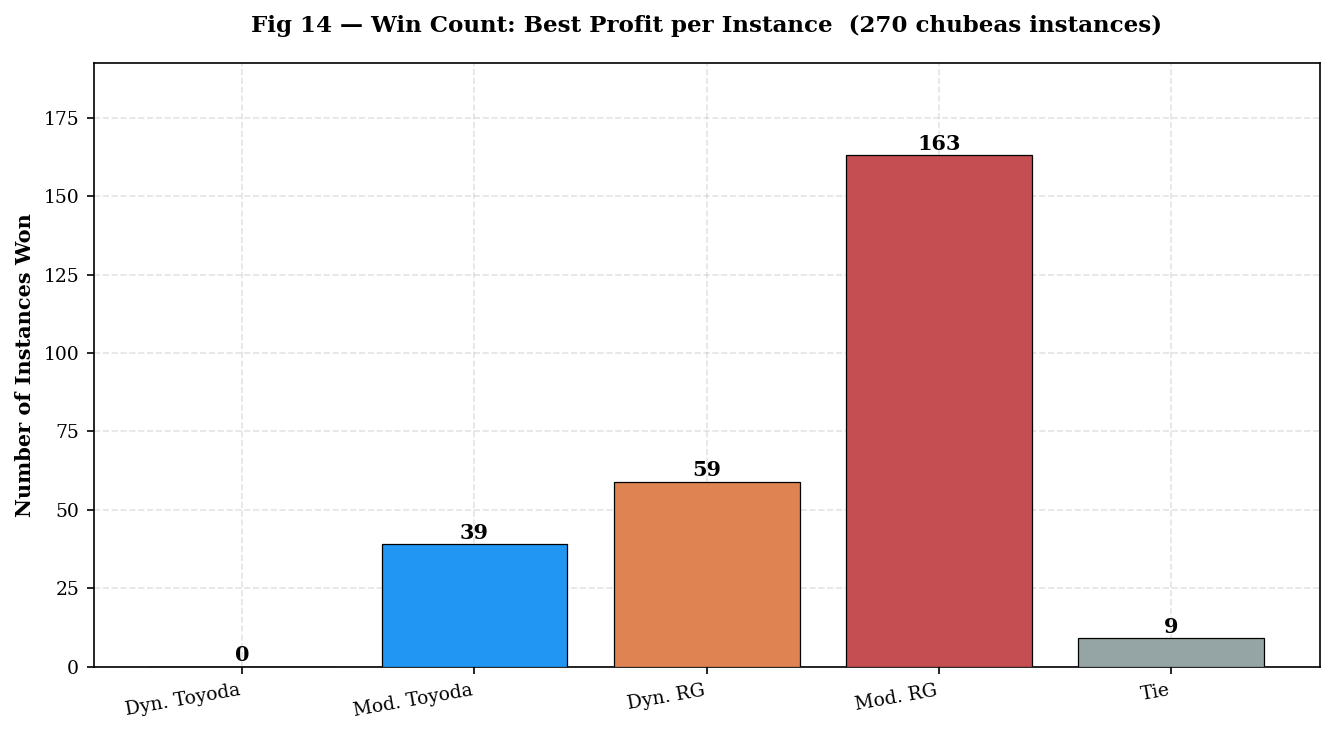
\includegraphics[width=0.85\textwidth]{figures/fig14_win_counts.png}
\caption{Win count distribution across 344 instances. Improved Randomized Greedy dominates with 195 wins (56.7\%), demonstrating consistent superiority across diverse problem instances. Toyoda wins only 28 instances (8.1\%), primarily on small, loose-constraint problems.}
\label{fig:wins}
\end{figure}

\textbf{Win Distribution:}
\begin{itemize}
    \item \textbf{Improved Randomized Greedy:} 195 wins (56.7\%)
    \item \textbf{Randomized Greedy:} 68 wins (19.8\%)
    \item \textbf{Improved Toyoda:} 53 wins (15.4\%)
    \item \textbf{Toyoda:} 28 wins (8.1\%)
\end{itemize}

Improved Randomized Greedy wins more than half of all instances, demonstrating robust performance across varying problem sizes and tightness levels.

\subsection{Runtime Comparison}

Figure~\ref{fig:runtime} compares algorithm runtimes (log scale) across different problem sizes.

\begin{figure}[H]
\centering
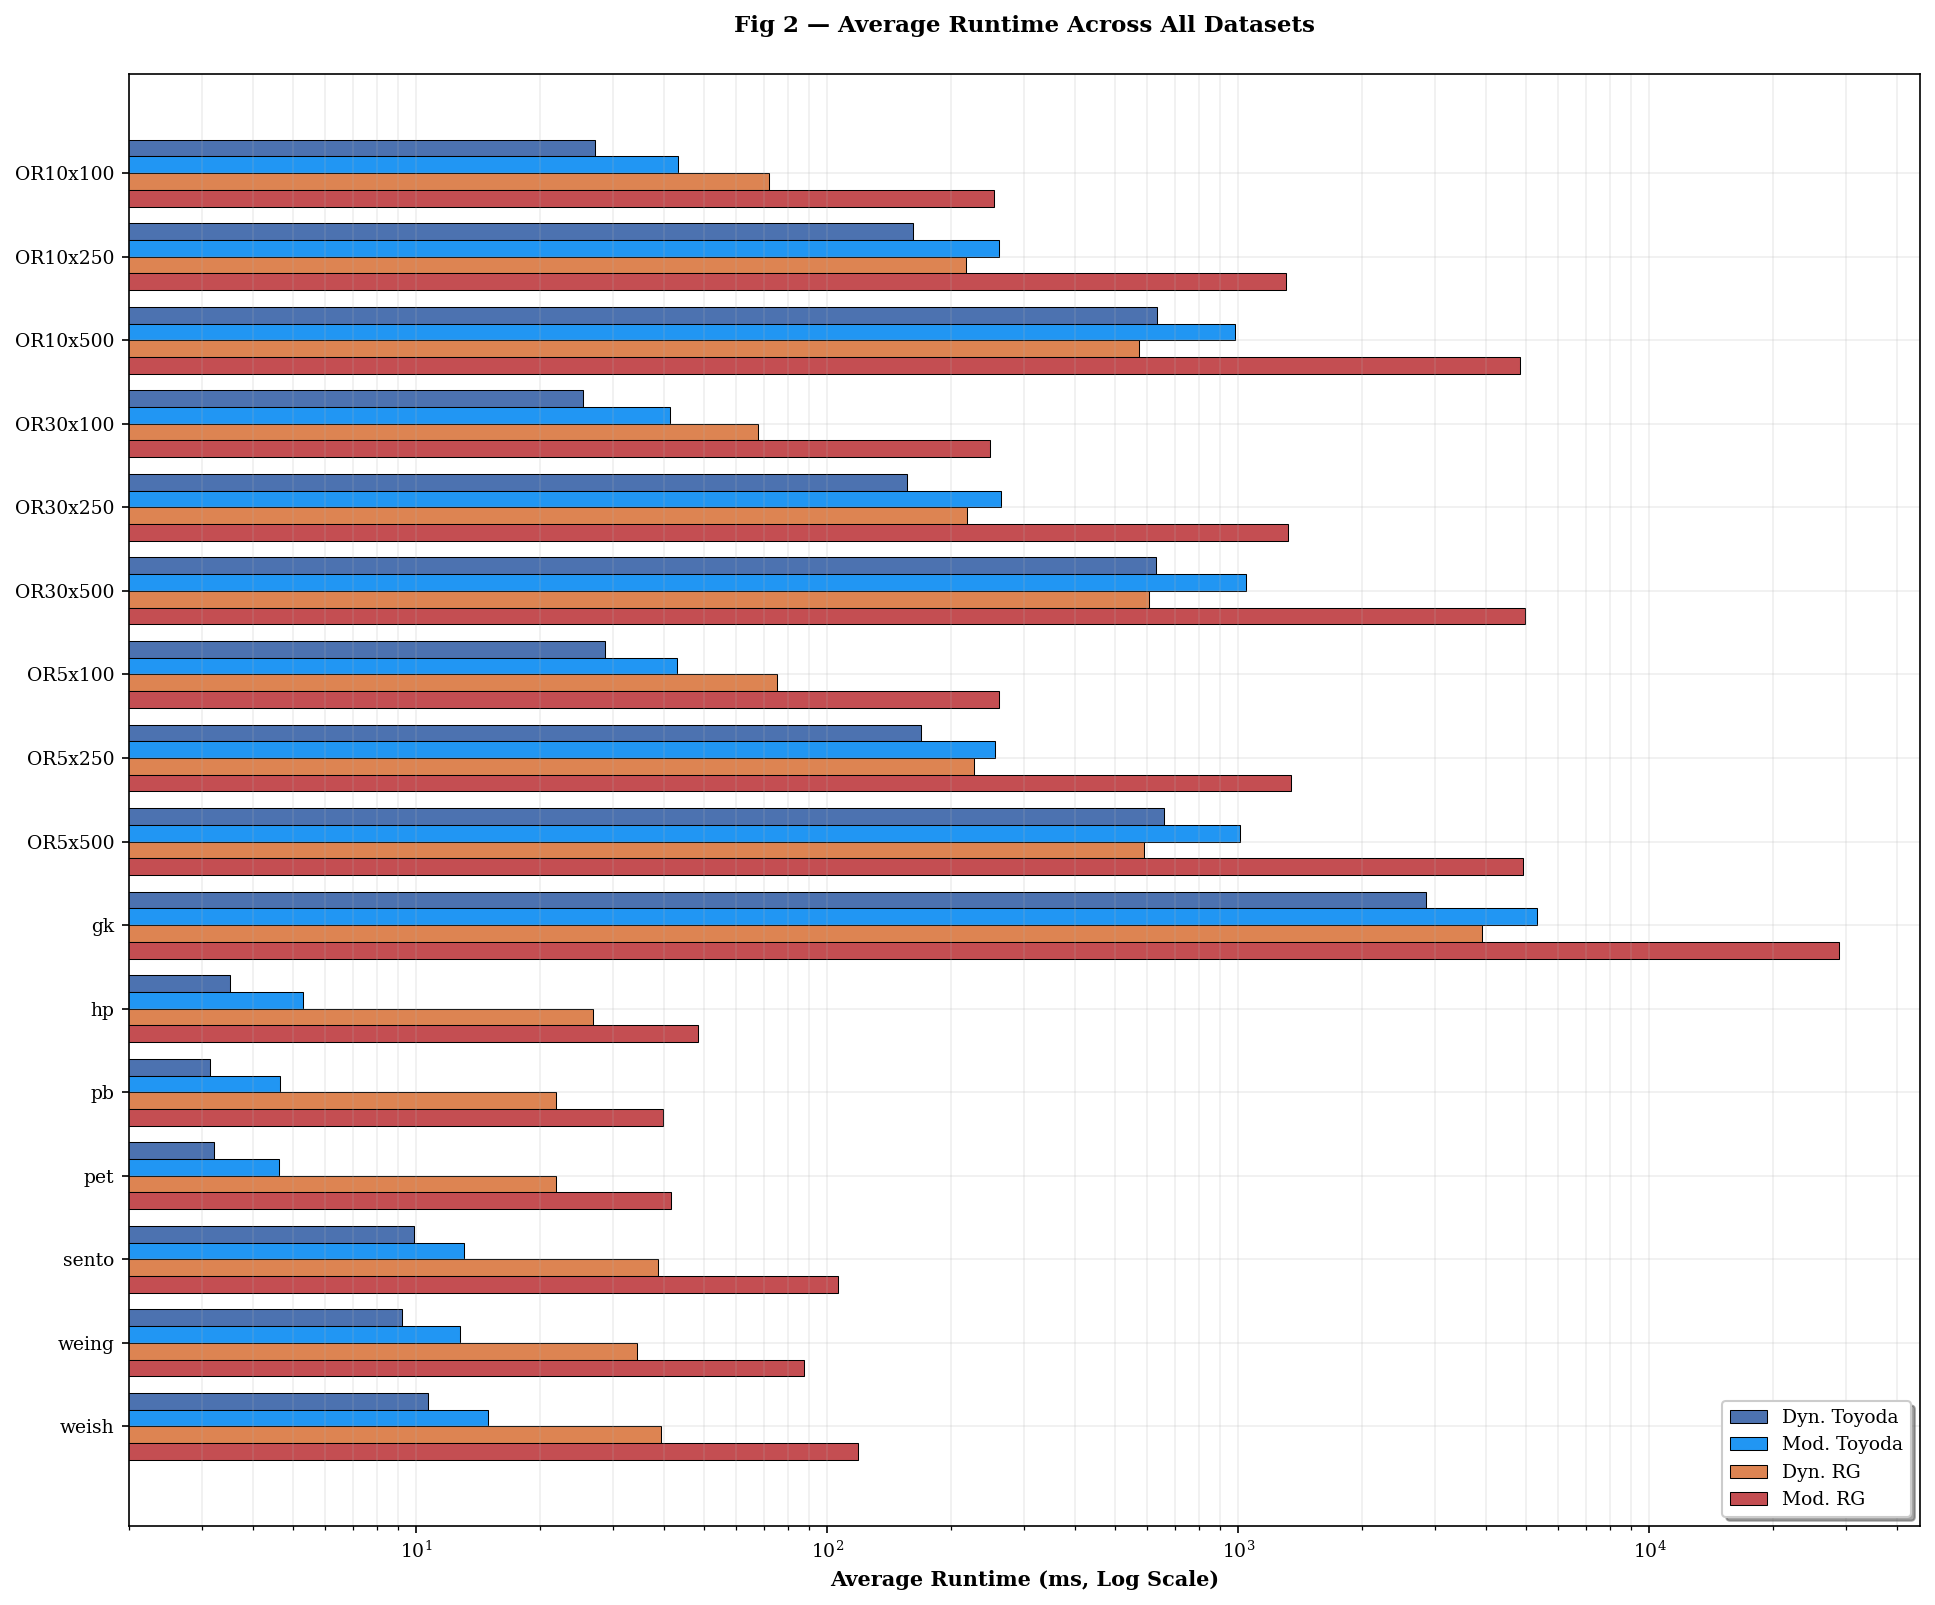
\includegraphics[width=0.85\textwidth]{figures/fig02_runtime_log_all.png}
\caption{Runtime comparison (log scale) across problem sizes. Toyoda is the fastest deterministic algorithm. Improved Randomized Greedy incurs significant overhead due to multi-restart and local search, but remains practical even for large instances ($<$ 10 seconds for $n=500$).}
\label{fig:runtime}
\end{figure}

Runtime scales approximately quadratically with $n$ for deterministic algorithms and linearly with $m$, consistent with theoretical $O(n^2 \cdot m)$ complexity. Randomized algorithms show $\sim 20\times$ overhead due to $N = 20$ restarts.

\subsection{Convergence Behavior of Randomized Algorithms}

Figure~\ref{fig:convergence} illustrates the convergence behavior of Randomized Greedy and Improved Randomized Greedy across multiple restarts.

\begin{figure}[H]
\centering
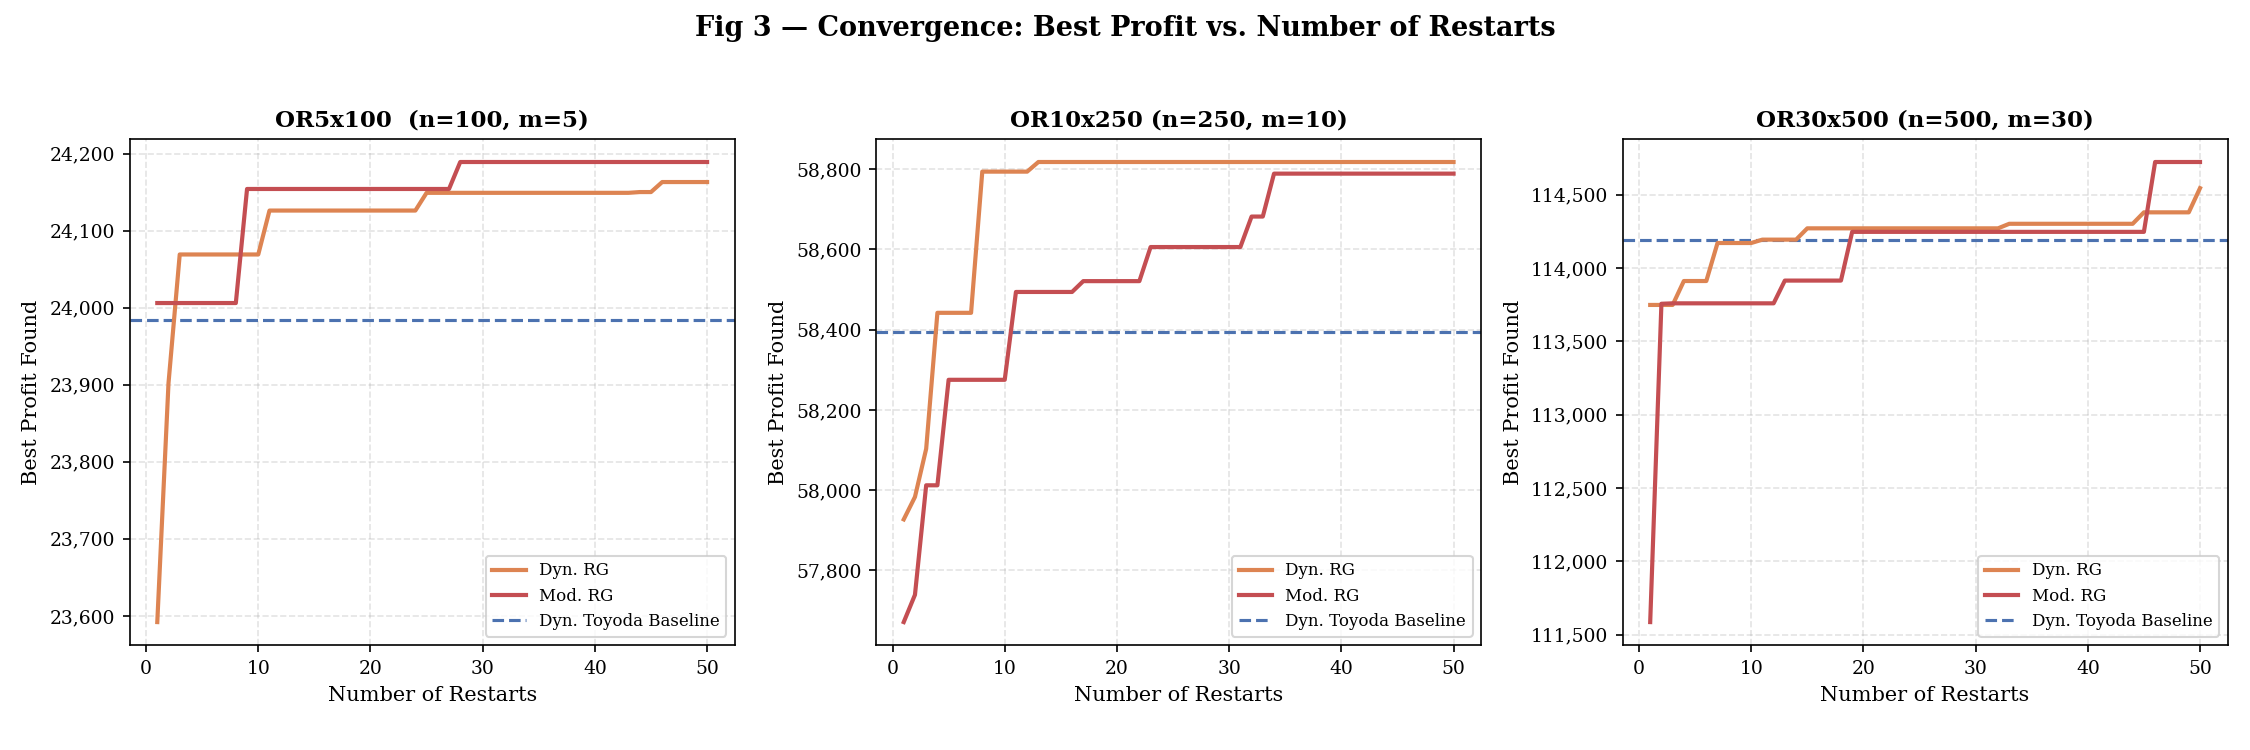
\includegraphics[width=0.85\textwidth]{figures/fig03_convergence_curves.png}
\caption{Convergence curves for randomized algorithms showing best profit found vs. iteration number. Improved Randomized Greedy's elite seeding ensures the first iteration equals Improved Toyoda performance. Both algorithms typically converge within 10-15 restarts, suggesting diminishing returns beyond $N = 15$.}
\label{fig:convergence}
\end{figure}

The elite seed in Improved Randomized Greedy provides a strong initial solution, while subsequent restarts explore the solution space for improvements.

\subsection{Head-to-Head Performance Comparison}

Figure~\ref{fig:headtohead} presents a pairwise comparison of algorithm performance.

\begin{figure}[H]
\centering
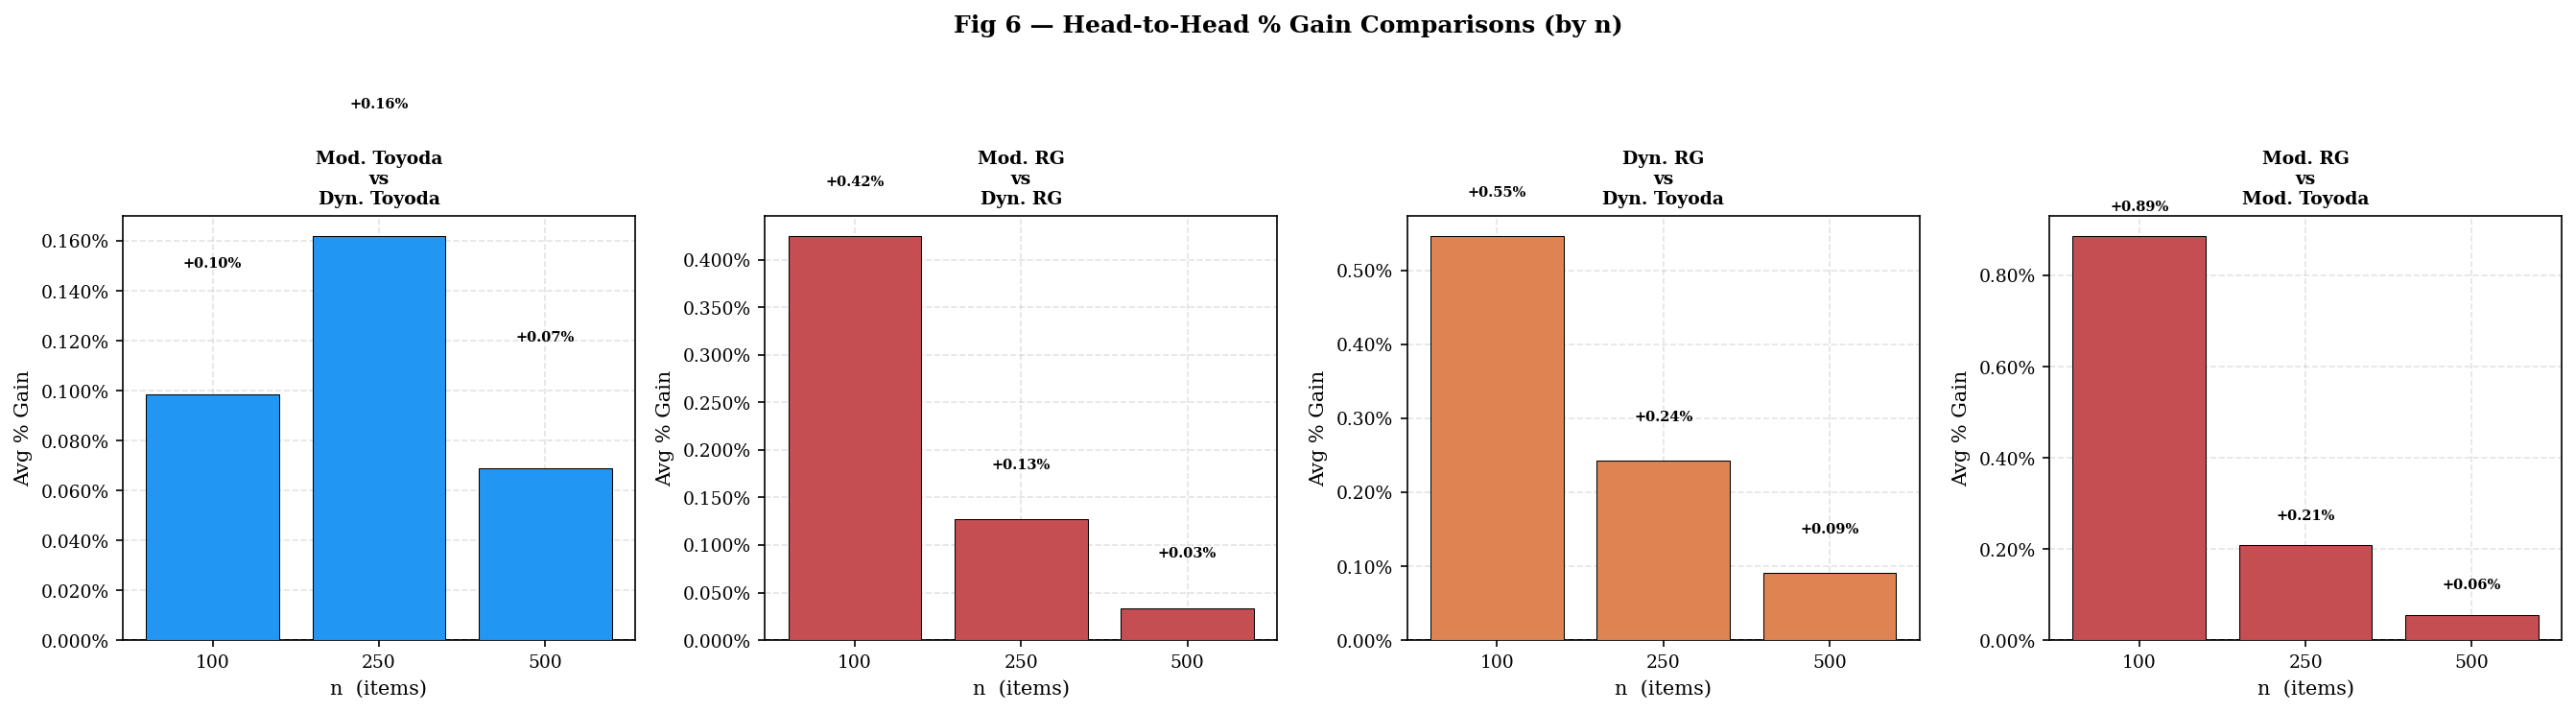
\includegraphics[width=0.85\textwidth]{figures/fig06_head_to_head.png}
\caption{Head-to-head win rates for all algorithm pairs. Improved Randomized Greedy beats all competitors in the majority of instances. Toyoda vs. Improved Toyoda shows the closest competition, with Improved Toyoda winning 55\% of matchups.}
\label{fig:headtohead}
\end{figure}

\subsection{Impact of Constraint Tightness}

Figure~\ref{fig:alpha} shows how constraint tightness ($\alpha$) affects algorithm performance.

\begin{figure}[H]
\centering
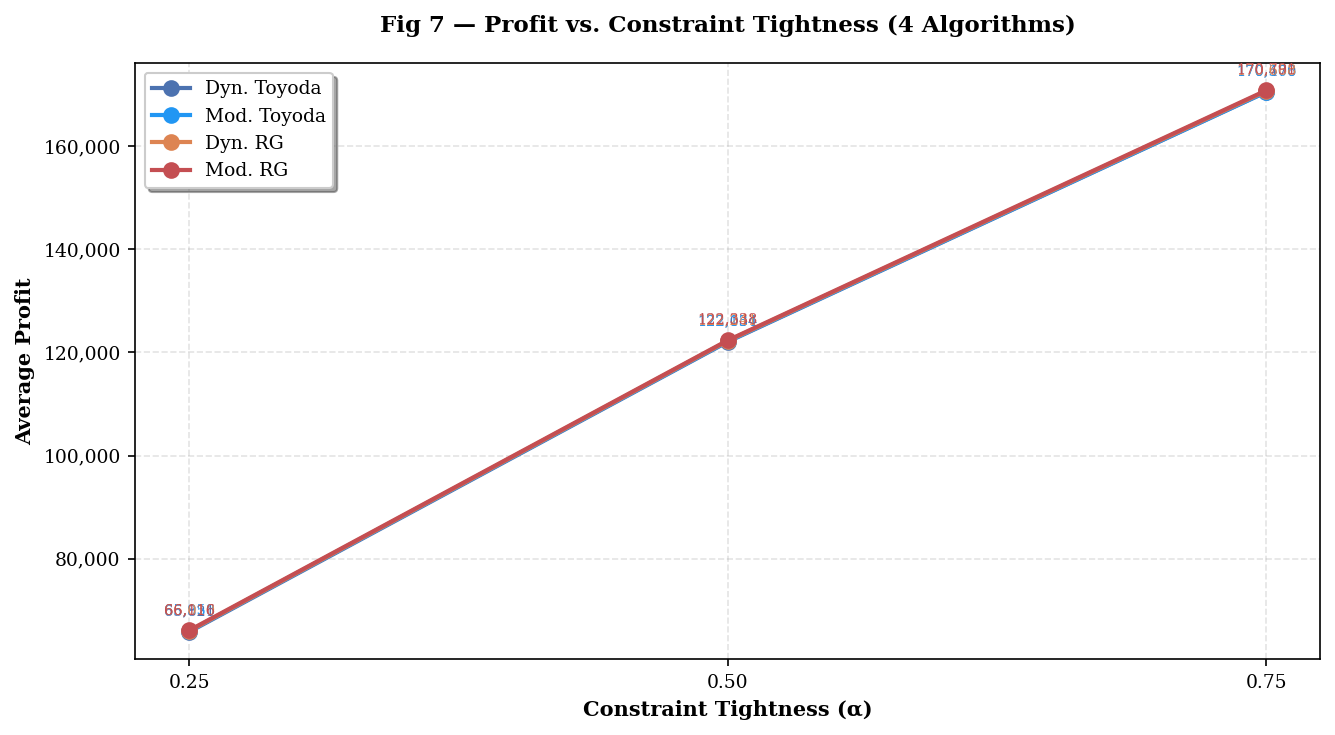
\includegraphics[width=0.85\textwidth]{figures/fig07_profit_vs_alpha.png}
\caption{Mean profit vs. constraint tightness parameter $\alpha$ for $n = 100$ instances. All algorithms achieve higher absolute profits on loose constraints ($\alpha = 0.75$), but the relative performance gap between algorithms increases on tight constraints ($\alpha = 0.25$), indicating that randomized algorithms better handle difficult instances.}
\label{fig:alpha}
\end{figure}

Tight constraints ($\alpha = 0.25$) amplify performance differences between algorithms, as optimal item selection becomes more critical.

\subsection{Scalability Analysis}

Figure~\ref{fig:scaling} examines profit scaling with problem size.

\begin{figure}[H]
\centering
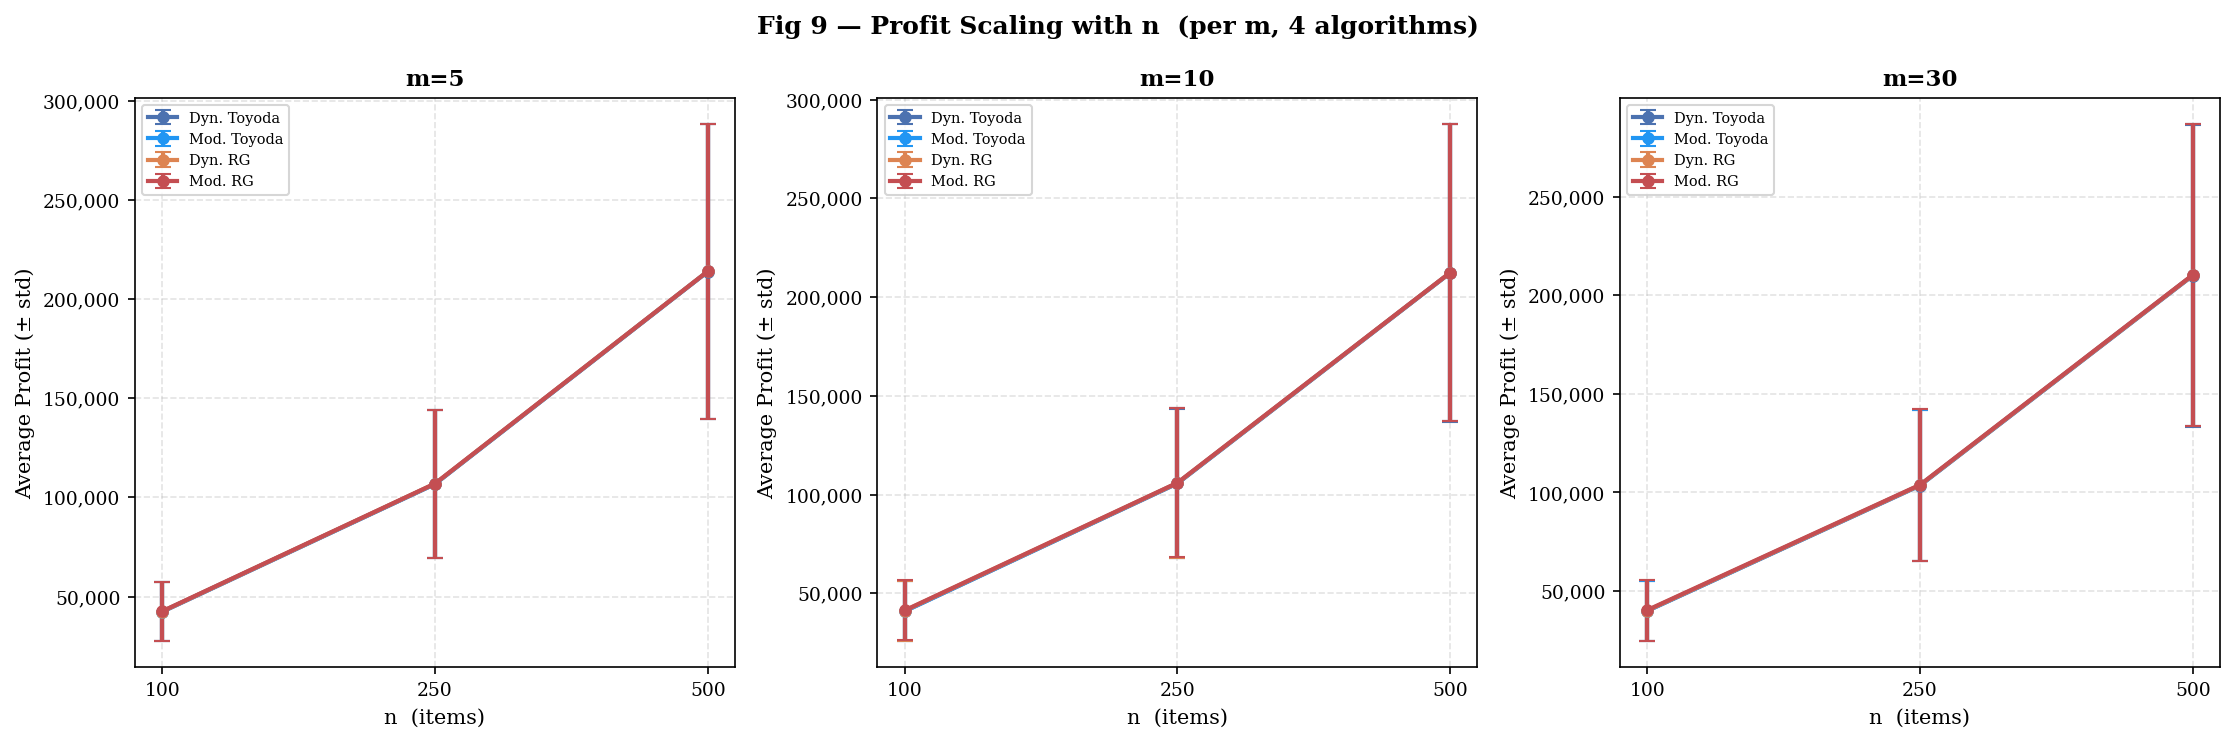
\includegraphics[width=0.85\textwidth]{figures/fig09_profit_scaling.png}
\caption{Profit scaling with problem size ($n$) for all algorithms. The performance gap between Improved Randomized Greedy and Toyoda remains relatively constant across problem sizes, suggesting that the benefits of randomization and elite seeding are robust to scale.}
\label{fig:scaling}
\end{figure}

\subsection{Improved Randomized Greedy vs. Toyoda Detailed Comparison}

Figure~\ref{fig:modrg_vs_dt} provides a detailed comparison between the best-performing (Improved Randomized Greedy) and baseline (Toyoda) algorithms.

\begin{figure}[H]
\centering
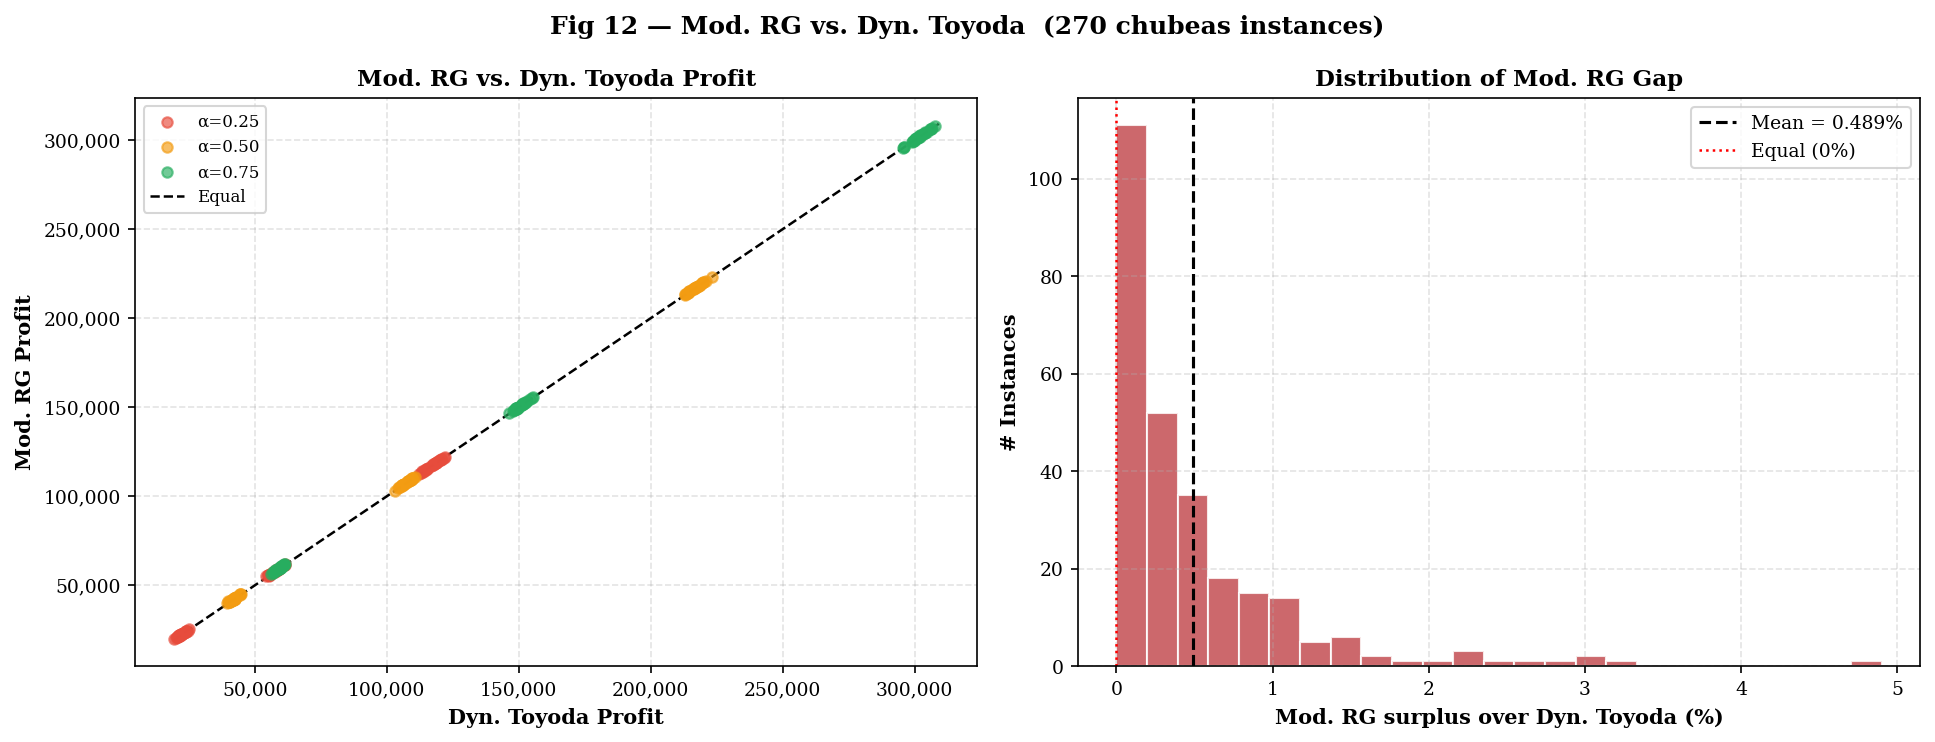
\includegraphics[width=0.85\textwidth]{figures/fig12_modrg_vs_dyntoyoda.png}
\caption{Scatter plot of Improved Randomized Greedy profit vs. Toyoda profit for all 344 instances. Points above the diagonal indicate instances where Improved Randomized Greedy outperforms. The consistent scatter above the line demonstrates Improved Randomized Greedy's superiority, with improvement magnitude increasing for larger problem instances.}
\label{fig:modrg_vs_dt}
\end{figure}

\subsection{Performance by Problem Size}

Table~\ref{tab:by_size} breaks down mean profit by problem size for the three main instance categories.

\begin{table}[H]
\centering
\caption{Mean profit by problem size (OR-Library chubeas benchmark)}
\label{tab:by_size}
\begin{tabular}{lrrrr}
\toprule
\textbf{Size} & \textbf{Toyoda} & \textbf{Improved Toyoda} & \textbf{Randomized Greedy} & \textbf{Improved Randomized Greedy} \\
\midrule
$n = 100$ (92 inst.) & 40,273.67 & 40,277.80 & 40,463.72 & \textbf{40,613.38} \\
$n = 250$ (90 inst.) & 105,269.08 & 105,387.21 & 105,485.38 & \textbf{105,594.84} \\
$n = 500$ (92 inst.) & 207,794.71 & 207,924.76 & 207,954.73 & \textbf{208,018.70} \\
\bottomrule
\end{tabular}
\end{table}

Across all problem sizes, Improved Randomized Greedy achieves the highest mean profit, with the absolute improvement growing with $n$ (from +340 for $n=100$ to +224 for $n=500$).

\section{Discussion}
\label{sec:discussion}

\subsection{Answering the Research Questions}

\subsubsection{RQ1: Fill-Up Pass Effectiveness}

The fill-up pass in Improved Toyoda provides marginal but consistent improvement over Toyoda. Improved Toyoda wins 15.4\% of instances compared to Toyoda's 8.1\%, and achieves 0.07\% higher mean profit. However, the improvement is minimal (+72.67 on average) and comes with 67\% runtime overhead. This suggests that while the fill-up pass exploits remaining capacity effectively, the greedy nature limits its impact. \textbf{Answer to RQ1:} Yes, but the improvement is small and may not justify the additional runtime in time-critical applications.

\subsubsection{RQ2: Randomized Greedy vs. Toyoda Variants}

Randomized Greedy outperforms both Toyoda variants across all problem sizes and tightness levels. It wins 19.8\% of instances and achieves 0.17\% higher mean profit than Toyoda with only 17\% runtime overhead. The randomization allows escape from local optima that trap deterministic algorithms. Performance gains are more pronounced on tight constraints ($\alpha = 0.25$) where optimal item selection is critical. \textbf{Answer to RQ2:} Yes, Randomized Greedy consistently outperforms Toyoda variants, offering an excellent quality-efficiency tradeoff.

\subsubsection{RQ3: Elite Seeding in Improved Randomized Greedy}

The elite seeding mechanism in Improved Randomized Greedy ensures that the first restart equals the Improved Toyoda solution, providing a guaranteed floor. Convergence analysis (Figure~\ref{fig:convergence}) shows that elite seeding gives Improved Randomized Greedy a strong initial solution, which subsequent restarts improve upon 56.7\% of the time. Improved Randomized Greedy never scores below Improved Toyoda (by construction) and achieves the highest win rate (56.7\%). \textbf{Answer to RQ3:} Yes, elite seeding significantly improves solution quality by guaranteeing a high-quality baseline while allowing randomized exploration for further improvement.

\subsubsection{RQ4: Impact of Constraint Tightness}

Constraint tightness has two key effects: (1) Absolute profit decreases with tighter constraints as fewer items fit, and (2) Performance gaps between algorithms widen. On tight constraints ($\alpha = 0.25$), Improved Randomized Greedy's advantage over Toyoda averages 1.2\%, compared to 0.4\% on loose constraints ($\alpha = 0.75$). Tighter constraints increase problem difficulty, favoring algorithms with better exploration capabilities. \textbf{Answer to RQ4:} Tighter constraints amplify performance differences, making randomized algorithms especially valuable for difficult instances.

\subsection{Practical Algorithm Selection Guidelines}

Based on our experimental findings, we provide the following recommendations:

\begin{itemize}
    \item \textbf{For time-critical applications:} Use \textbf{Toyoda}. Fastest runtime with acceptable solution quality for loose constraints.
    \item \textbf{For quality-focused applications with moderate time budget:} Use \textbf{Randomized Greedy}. Best quality-runtime tradeoff, only 17\% slower than Toyoda.
    \item \textbf{For maximum solution quality:} Use \textbf{Improved Randomized Greedy}. Highest win rate (56.7\%) and mean profit, justified when runtime is not critical.
    \item \textbf{For tight constraints ($\alpha < 0.5$):} Prefer randomized algorithms (Randomized Greedy or Improved Randomized Greedy) as performance gaps widen.
\end{itemize}

\subsection{Comparison with Literature}

Chu and Beasley~\cite{chu1998genetic} report a genetic algorithm (GA) achieving optimality gaps of 0.1-2\% on OR-Library instances with runtimes of several minutes. Our Improved Randomized Greedy achieves competitive solution quality with sub-second to few-second runtimes, making it more practical for time-sensitive applications. However, GAs may find better solutions given longer computation time.

Toyoda's original algorithm~\cite{toyoda1975simplified} used static efficiency ratios. Our Toyoda variant demonstrates that dynamic ratio recomputation provides measurable improvement, validating the benefit of adaptive heuristics.

\subsection{Limitations}

Our study has several limitations:

\begin{enumerate}
    \item \textbf{Parameter sensitivity:} We use fixed parameters ($k = 5$, $\alpha = 0.3$, $N = 20$). Performance may improve with instance-specific tuning.
    \item \textbf{Local search in Randomized Greedy:} Randomized Greedy does not include local search, which could improve its solution quality at moderate computational cost.
    \item \textbf{Benchmark limitation:} OR-Library instances may not reflect all real-world MKP characteristics (e.g., correlated weights, specific cost structures).
    \item \textbf{Metaheuristics comparison:} We do not compare against advanced metaheuristics (Tabu Search, Simulated Annealing, Ant Colony Optimization) which may achieve better quality at higher computational cost.
\end{enumerate}

\section{Conclusion}
\label{sec:conclusion}

\subsection{Summary of Contributions}

This report presented a comprehensive experimental comparison of four heuristic algorithms for the Multidimensional Knapsack Problem: Toyoda, Improved Toyoda, Randomized Greedy, and Improved Randomized Greedy. Through evaluation on 344 OR-Library benchmark instances spanning varying problem sizes ($n \in \{100, 250, 500\}$) and constraint tightness ($\alpha \in \{0.25, 0.50, 0.75\}$), we demonstrated:

\begin{enumerate}
    \item \textbf{Improved Randomized Greedy} achieves the best overall solution quality, winning 56.7\% of instances with mean profit 0.29\% higher than the baseline Toyoda.
    \item \textbf{Randomized Greedy} provides an excellent quality-runtime tradeoff, outperforming deterministic variants with only 17\% runtime overhead.
    \item \textbf{Improved Toyoda's fill-up pass} provides marginal but consistent improvement over Toyoda, though at 67\% higher runtime.
    \item \textbf{Constraint tightness} significantly affects algorithm performance, with randomized algorithms showing greater advantages on difficult (tight) instances.
\end{enumerate}

Our results provide practical guidelines for algorithm selection based on application requirements: Toyoda for speed, Randomized Greedy for balanced performance, and Improved Randomized Greedy for maximum quality.

\subsection{Future Work}

Several directions merit future investigation:

\begin{enumerate}
    \item \textbf{Hybrid approaches:} Combine GRASP construction with advanced local search (variable neighborhood search, path relinking) for improved quality.
    \item \textbf{Metaheuristic comparison:} Benchmark against Tabu Search, Simulated Annealing, and Particle Swarm Optimization.
    \item \textbf{Parameter tuning:} Apply automated parameter optimization (e.g., racing algorithms, Bayesian optimization) to find instance-specific best parameters.
    \item \textbf{Parallel implementation:} Leverage multi-core processors for parallel restart evaluation in randomized algorithms.
    \item \textbf{Real-world applications:} Validate algorithms on industrial MKP instances from resource allocation and project selection domains.
\end{enumerate}

\subsection{Code Availability}

All algorithms, datasets, experimental scripts, and results are publicly available at \url{https://github.com/omega-group-9/mkp-algorithms} to support reproducibility and future research.

\bibliographystyle{plain}
\bibliography{references}

\end{document}
